% !TEX TS-program = pdflatex
% !TEX encoding = UTF-8 Unicode

% This is a simple template for a LaTeX document using the "article" class.
% See "book", "report", "letter" for other types of document.

\documentclass[11pt]{article} % use larger type; default would be 10pt

\usepackage[utf8]{inputenc} % set input encoding (not needed with XeLaTeX)

%%% Examples of Article customizations
% These packages are optional, depending whether you want the features they provide.
% See the LaTeX Companion or other references for full information.

%%% PAGE DIMENSIONS
\usepackage{geometry} % to change the page dimensions
\geometry{a4paper} % or letterpaper (US) or a5paper or....
% \geometry{margin=2in} % for example, change the margins to 2 inches all round
% \geometry{landscape} % set up the page for landscape
%   read geometry.pdf for detailed page layout information

\usepackage{graphicx} % support the \includegraphics command and options

% \usepackage[parfill]{parskip} % Activate to begin paragraphs with an empty line rather than an indent

%%% PACKAGES
\usepackage{booktabs} % for much better looking tables
\usepackage{array} % for better arrays (eg matrices) in maths
\usepackage{paralist} % very flexible & customisable lists (eg. enumerate/itemize, etc.)
\usepackage{verbatim} % adds environment for commenting out blocks of text & for better verbatim
\usepackage{subfig} % make it possible to include more than one captioned figure/table in a single float
\usepackage{listings} % used to write pieces of code
\usepackage{xcolor}
\usepackage{hyperref} % used to generate external links
% These packages are all incorporated in the memoir class to one degree or another...

%%% HEADERS & FOOTERS
\usepackage{fancyhdr} % This should be set AFTER setting up the page geometry
\pagestyle{fancy} % options: empty , plain , fancy
\renewcommand{\headrulewidth}{0pt} % customise the layout...
\lhead{}\chead{}\rhead{}
\lfoot{}\cfoot{\thepage}\rfoot{}

%%% SECTION TITLE APPEARANCE
\usepackage{sectsty}
\allsectionsfont{\sffamily\mdseries\upshape} % (See the fntguide.pdf for font help)
% (This matches ConTeXt defaults)

%%% ToC (table of contents) APPEARANCE
\usepackage[nottoc,notlof,notlot]{tocbibind} % Put the bibliography in the ToC
\usepackage[titles,subfigure]{tocloft} % Alter the style of the Table of Contents
\renewcommand{\cftsecfont}{\rmfamily\mdseries\upshape}
\renewcommand{\cftsecpagefont}{\rmfamily\mdseries\upshape} % No bold!

%%% END Article customizations

%%% The "real" document content comes below...

\title{Prova Finale - Reti Logiche (prof. William Fornaciari)}
\author{Corigliano Emilio 10627041 - 907936}
\date{A.A. 2020/21} % Activate to display a given date or no date (if empty)

\begin{document}
\maketitle

\section{Introduzione e spiegazione del problema}
Il progetto consiste nella progettazione di un circuito per l'equalizzazione di immagini in scala di grigi a 256 valori mediante il linguaggio di definizione hardware VHDL, attraverso il software \textit{Vivado}. L'equalizzazione è un processo di elaborazione digitale che consiste nell'elaborare l'immagine affinchè i suoi colori coprano tutto lo spettro disponibile. Nel nostro caso, dopo l'elaborazione vogliamo ottenere delle immagini che abbiano pixel di valore 0 e 255 rispettivamente nei punti di valore minimo e massimo nell'immagine originale; tutti gli altri pixel verranno ridistribuiti su tutto lo spettro in maniera coerente.

\begin{figure}[h!]
\centering
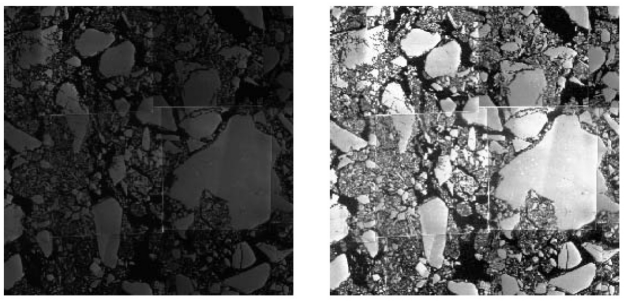
\includegraphics[width=120mm]{esempio-di-equalizzazione.png}
\caption{esempio di equalizzazione di un'immagine}
\end{figure}

\section{Considerazioni, approccio e scelte implementative}

Leggendo la specifica si possono fare delle prime considerazioni generali, per poi approfondire ogni aspetto particolare:
\begin{itemize}
\item Non è necessario distinguere le varie righe, si può trattare la memoria semplicemente come un vettore di dimensione $N = R \cdot C$ da analizzare sequenzialmente;
\item Per le scansioni dell'immagine si è scelto di utilizzare un contatore che contasse $N$ cicli di clock; Questo ha lo svantaggio di dover essere computato in una fase a sè antecedente alle altre ma il vantaggio di poter avere una corrispondenza immediata tra il contatore ($i$) e gli indirizzi di memoria da leggere ($2+i$) o scrivere ($2+N+i$), con $i \in [0, N)$;
\item È necessario che si scansioni preliminarmente una volta tutta l'immagine così da trovare i byte di valore massimo ($MAX\_PV$) e minimo ($MIN\_PV$); questa fase deve necessariamente essere precedente alla vera e propria elaborazione dell'immagine poichè quest'ultima ha bisogno dell'elaborazione dello $SHIFT\_VALUE$ (computato a partire dalla differenza tra $MAX\_PV$ e $MIN\_PV$).
\item Infine, è necessario eseguire un'altra scansione dell'immagine per eseguire la vera e propria elaborazione. 
\end{itemize}
 
\subsection{Registri}
Di seguito si elencano i diversi registri usati al fine di memorizzare importanti informazioni per l'elaborazione dell'immagine:
\begin{itemize}
\item $rN$: memorizza il numero totale di byte che compongono l'immagine
\item $rMax$: memorizza il valore massimo dei pixel presente nell'immagine
\item $rMin$: memorizza il valore minimo dei pixel presente nell'immagine	
\item $rSL$: memorizza lo $SHIFT\_LEVEL$ da adoperare per l'equalizzazione.
\end{itemize}
Altri registri sono stati usati per poter realizzare varie parti del componente:
\begin{itemize}
\item $r1$: è usato per memorizzare il numero da aggiungere ad ogni ciclo per l'algoritmo delle somme ripetute per il prodotto di $N = R \cdot C$;
\item $rC1$: è il registro che permette di contare quante volte eseguire l'operazione di somme ripetute per computare $N$;
\item $rC2$: è il registro che permette di contare l'indice per la valutazione del valore del pixel nella fase in cui si ricercano il valore massimo e minimo;
\item $rC3$: è il registro che permette di contare l'indice del pixel da elaborare;
\end{itemize}

\subsection{Fasi}
Ci sono 4 fasi fondamentali che occorre attraversare per elaborare l'immagine, ognuna delle quali ha bisogno di dati elaborati precedentemente. Per questo non sono ulteriormente parallelizzabili.

Si è scelto di affrontare ogni fase singolarmente per semplificare l'esposizione; questo approccio ha semplificato anche l'implementazione, di conseguenza le diverse fasi sono indipendenti tra loro. Seguendo questo metodo, però, si è limitata l'ottimizzazione del progetto, facendo sì che alcuni componenti (come per esempio i contatori o la dimensione di alcuni segnali) non fossero in numero o in dimensione minima ma rispecchiassero la volontà di fare un progetto più semplice da analizzare ed esporre. Questo approccio non è stato ritenuto un problema data la dimensione del progetto e la qualità dell'hardware per il quale è stato progettato; si è preferita la qualità e semplicità espositiva alla ottimizzazione progettuale.

\begin{figure}[h]
\centering
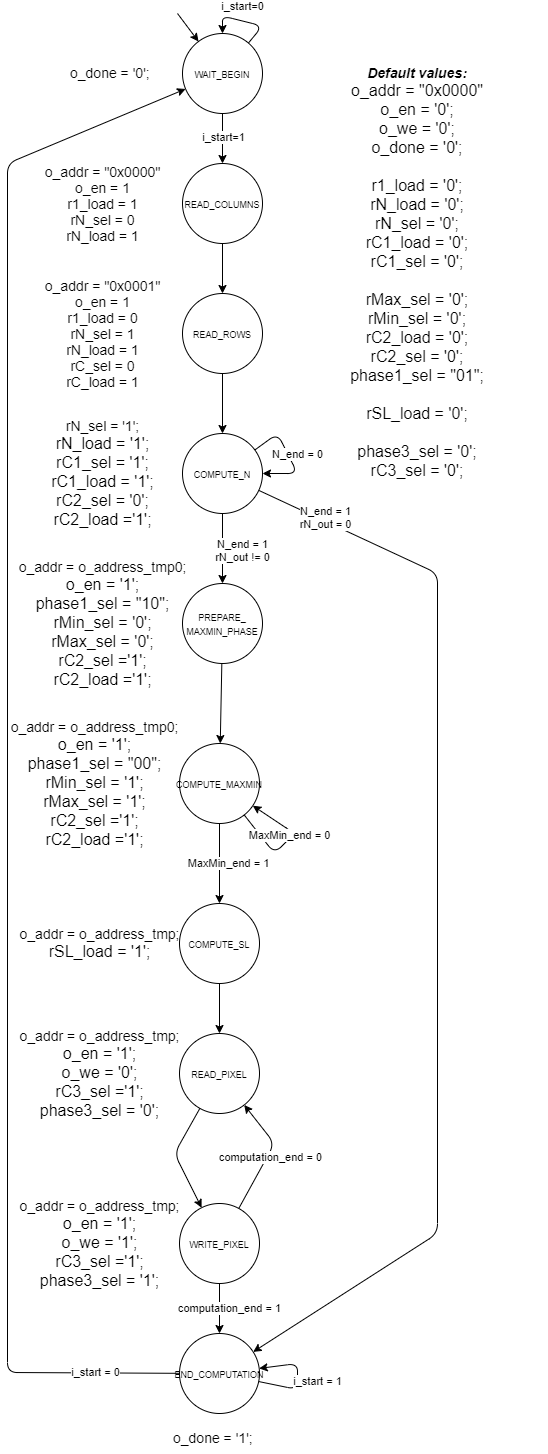
\includegraphics[scale=0.2995]{../datapaths/FSM-vertical.png}
\caption{FSM dell'elaborazione}
\end{figure}

\subsubsection{computazione della quantità di pixel}
La prima fase è quella in cui si calcola la dimensione dell'immagine $N$ da equalizzare. Questo valore è ottenuto moltiplicando $mem[0]$ e $mem[1]$ tramite un moltiplicatore per somme successive. Alla fine dell'operazione viene portato in alto il segnale $N\_end$ che indica la fine dell'operazione. Da questo momento fino alla prossima esecuzione nel registro $rN$ ci sarà il valore $N = R \cdot C$.

\begin{figure}[h]
\centering
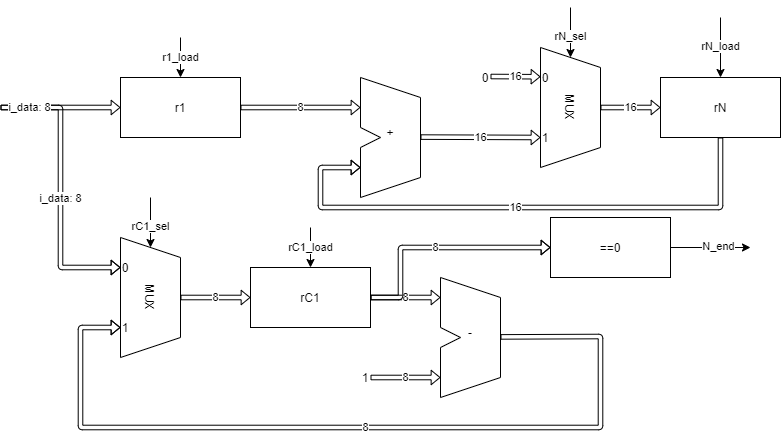
\includegraphics[width=120mm]{../datapaths/regN.png}
\caption{computazione della quantità di pixel}
\end{figure}


\subsubsection{Ricerca dei valori massimi e minimi dei pixel}
Nella seconda fase si cercano il valore massimo ($MAX\_PV$) e il valore minimo ($MIN\_PV$): si scorre una prima volta tutta l'immagine e si cercano contemporaneamente il valore massimo e minimo dei pixel presenti nell'immagine mediante confronto con il valore presente nel registro. I valori iniziali dei registri per il valore massimo e minimo sono rispettivamente $0$ e $255$, risultato che ovviamente non potrà mai rimanere invariato. Infatti in ogni esecuzione il primo pixel letto sarà maggiore o uguale del valore di default del registro $rMax$ e minore o uguale del valore di default del registro $rMin$. Per tenere conto dei pixel letti e per generare l'indirizzo al quale leggere il valore si usa un contatore che parte da 0 e ad ogni ciclo di clock incrementa di 1, fino a raggiungere $N$; a questo punto verrà portato in alto il segnale di $MaxMin\_end$.

\begin{figure}[h]
\centering
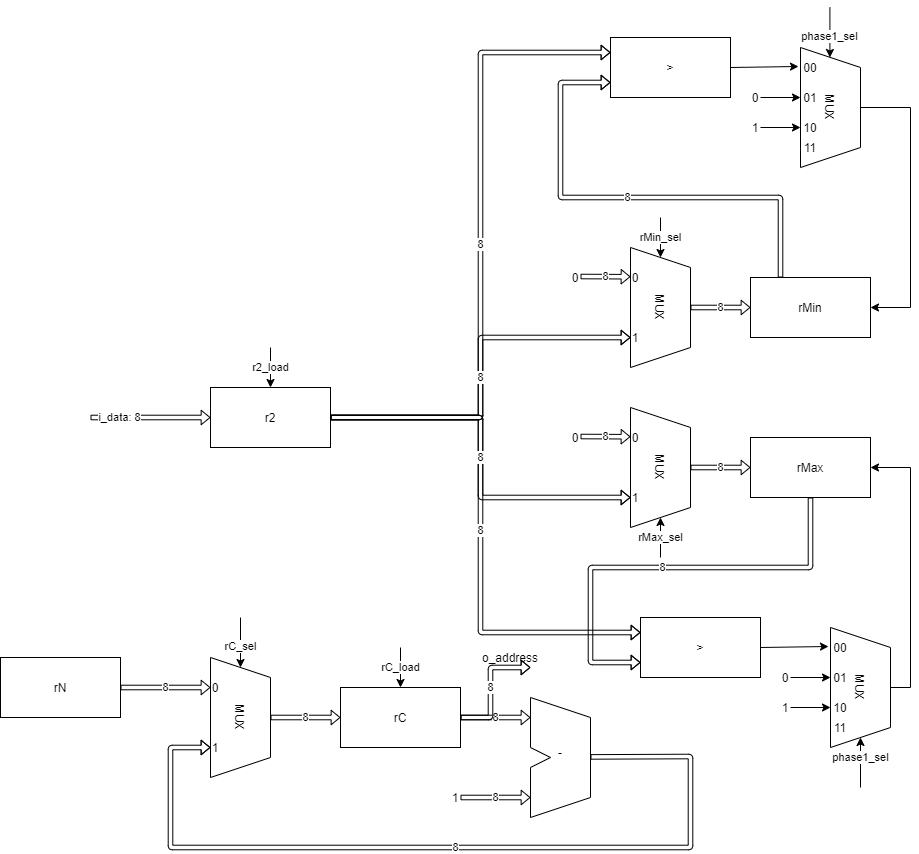
\includegraphics[width=120mm]{../datapaths/regMax_regMin.png}
\caption{Ricerca dei valori massimi e minimi dei pixel}
\end{figure}


\subsubsection{Computazione del valore SHIFT\_LEVEL}
La terza fase prevede il calcolo dello $SHIFT\_LEVEL$; questo viene ottenuto implementando una funzione combinatoria che esegue un controllo a soglie (nel diagramma rappresentata con il blocco $f(x)$ avente come input 8 bit e come output 4 bit). La funzione combinatoria prende in input $MAX\_PV - MIN\_PV + 1$ (quindi il $DELTA\_VALUE$ incrementato di 1) perchè si era pensato che sarebbe stato più semplice la generalizzazione. Infatti visualizzando gli shift level corrispondenti a tutti i valori di delta value possibili incrementati di uno (per esempio grazie allo script~\ref{lst:soglie}), si nota una semplice correlazione tra la posizione in cui compare il primo 1 e il valore dello $SHIFT\_LEVEL$ corrispondente.

\begin{lstlisting}[language=Python, caption=Generazione di soglie, label={lst:soglie}]
for i in range(256):
	print(bin(i) + ": " + str(8 - math.floor(math.log2(i+1))))
\end{lstlisting}

\begin{figure}[h]
\centering
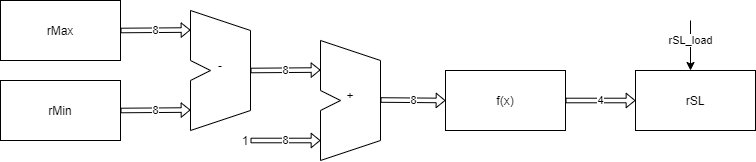
\includegraphics[width=120mm]{../datapaths/regSL_final.png}
\caption{Computazione dello shift level}
\end{figure}


\subsubsection{Equalizzazione}
La quarta fase, quella finale, provvede a equalizzare l'immagine tramite l'algoritmo fornitoci. Per ogni pixel che compone l'immagine (il cui indirizzo è computato grazie ad un contatore che parte da $N-1$ e decrementa fino a 0) si legge il valore originale. Al ciclo successivo si provvede a scrivere in memoria il valore computato all'indirizzo del pixel originale incrementato di $N$. Sono necessari due cicli per ogni pixel da equalizzare poichè la memoria prevede un solo segnale per codificare l'indirizzo su cui leggere o scrivere; visto che l'immagine originale non va sovrascritta si deve alternare una fase di lettura con una di scrittura, nelle quali cambierà $o\_address$.

\begin{figure}[h]
\centering
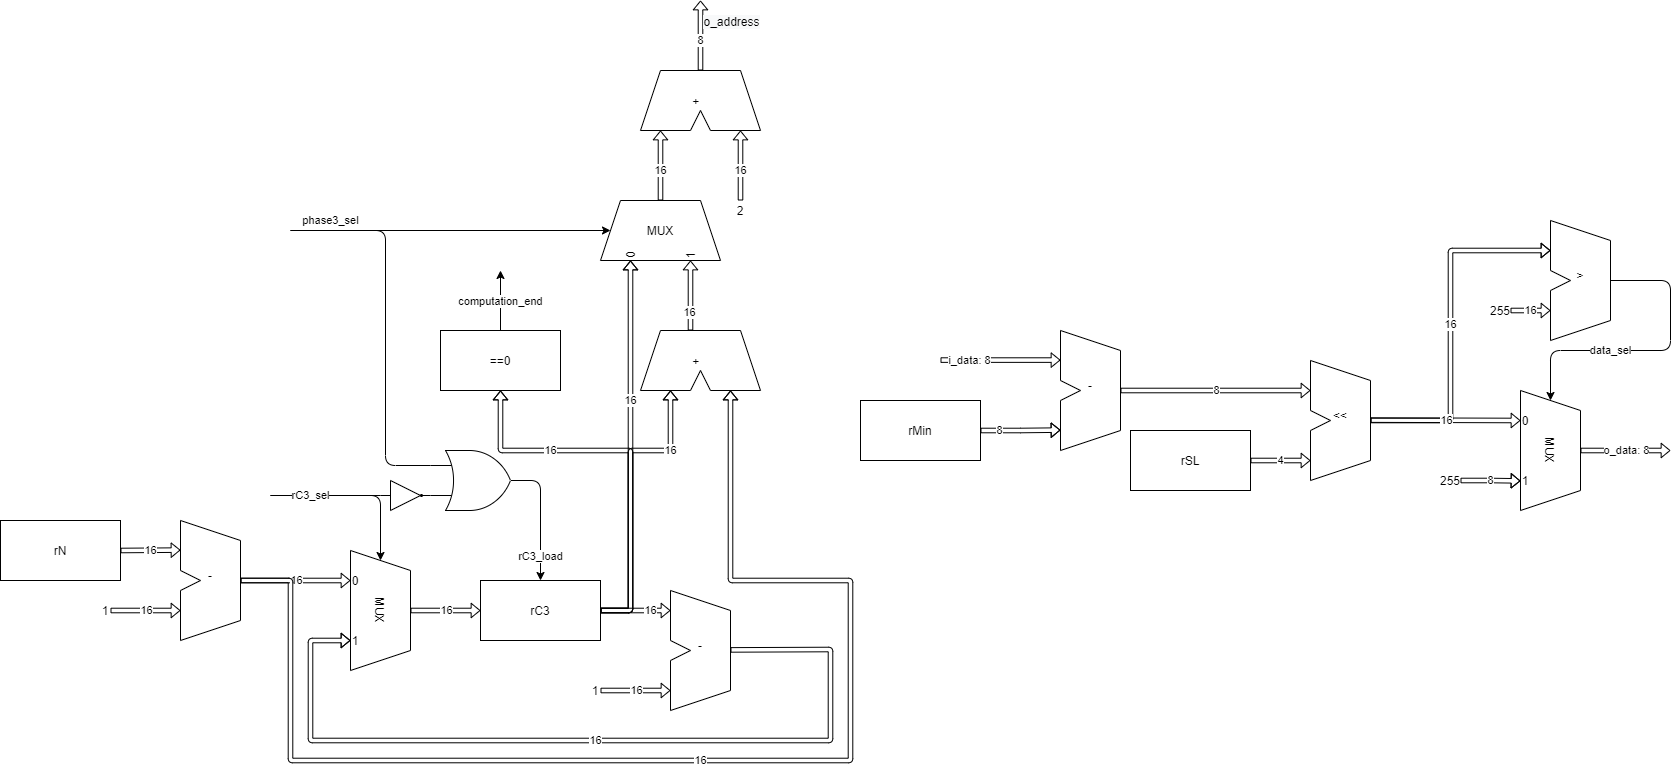
\includegraphics[width=120mm]{../datapaths/computation.png}
\caption{Equalizzazione}
\end{figure}

\subsubsection{Fine computazione}
La computazione finisce quando nello stato $WRITE\_PIXEL$ è alto il segnale $computation\_end$ oppure se alla fine dell'elaborazione del valore $N$ questo è $0$. Raggiunto lo stato di $END\_COMPUTATION$ si alza $o\_done$ e si aspetta in questo stato fintantoché $i\_start$ è alto. Quando questo segnale viene abbassato si ritorna allo stato $WAIT\_BEGIN$ e si riabbassa $o\_done$. Una nuova esecuzione partirà quando viene alzato di nuovo il segnale $i\_start$.


\section{Risultati}
Il componente è stato sviluppato, sintetizzato e testato sia con simulazioni behavioural che post-synthetis.

\subsection{testing}
Per testare il componente sviluppato sono stati scritti (con l'aiuto di script in python) dei testbanch. La maggior parte dei test con input random sono stati creati grazie ad un \href{https://github.com/davidemerli/RL-generator-2020-2021.git}{generatore di test} disponibile pubblicamente. Tutti gli altri test sono stati creati con un generatore custom che permetteva di creare dei testbanch a partire da configurazioni particolari della memoria scritte a mano così da controllare dei corner-cases o dei punti critici del codice. Di seguito sono leggermente approfonditi vari testbanch usati sul componente:

\begin{itemize}
\item dati casuali: centinaia di test sono stati implementati con dimensione e immagine iniziale casuali; in questi si includono anche tutti i testbanch fornitoci in allegato alla specifica. 
\item immagini grandi: vari test con dimensione dell'immagine molto grande (di cui uno con dimensione 128x128, cioè la dimensione massima) e immagine generata casualmente; questo serve a testare in particolar modo se le dimensioni dei collegamenti tra i vari componenti sono sufficientemente grandi e se la fase di calcolo della dimensione dell'immagine gestisce il caso limite della dimensione massima.
\item immagine di un pixel: test per analizzare il comportamento nel caso in cui ci sia solo un pixel;
\item zero righe o zero colonne: due test per provare il funzionamento del componente se un dato tra righe o colonne è 0. Utile per testare un caso limite per la fase di calcolo della dimensione dell'immagine;
\item stesso valore in tutta l'immagine: usato per testare il comportamento nel caso di un solo valore uguale per tutti i pixel dell'immagine. Sollecita un corner case nel calcolo dello $SHIFT\_LEVEL$;
\item valori immagine da 0 a 255: sollecita un altro corner case nel calcolo dello $SHIFT\_LEVEL$
\item più immagini consecutive: testato il caso in cui ci sono più immagini consecutive, la seconda caricata in memoria dopo la prima elaborazione e così via
\end{itemize}

\subsection{Report di sintesi}
Analizzando il report post sintesi sui timing si evince che il componente rispetta i constraints imposti: lo slack è di $5.239ns$ ed è positivo, quindi i constraints (di $10ns$ di clock) sono soddisfatti. I segnali si assestano dopo appena $4.610ns$, questo ci suggerisce che il componente potrebbe tranquillamente funzionare al doppio della frequenza, lasciando comunque margine per far stabilizzare tutte le uscite prima della fine del ciclo di clock. Inoltre, analizzando il report sugli utilizzi, non si trovano latch inferiti.

%\section{Conclusioni}

\end{document}